\documentclass[12pt,a4paper]{article}

% ============================================================
% PACKAGES
% ============================================================
\usepackage[a4paper,margin=1in]{geometry}
\usepackage[T1]{fontenc}
\usepackage{times}
\usepackage{microtype}
\usepackage{setspace}
\usepackage{graphicx}
\usepackage{float}
\usepackage{booktabs}
\usepackage{array}
\usepackage{multirow}
\usepackage{longtable}
\usepackage{tabularx}
\usepackage{makecell}
\usepackage{seqsplit}
\usepackage{amsmath,amssymb}
\usepackage{algorithm}
\usepackage{algpseudocode}
\usepackage{xcolor}
\usepackage{listings}
\usepackage{tikz}
\usepackage{pgfplots}
\usepackage{caption}
\usepackage{subcaption}
\usepackage{hyperref}
\usepackage{enumitem}
\usepackage{fancyhdr}
\usepackage{titlesec}

\usetikzlibrary{
    shapes.geometric,
    arrows.meta,
    positioning,
    fit,
    calc,
    decorations.pathreplacing
}

\pgfplotsset{compat=1.18}

% ============================================================
% HYPERLINKS
% ============================================================
\hypersetup{
    colorlinks=true,
    linkcolor=teal,
    citecolor=blue,
    urlcolor=teal,
    pdftitle={Intelligent Compiler for Detecting Errors in Genomic Data Processing Pipelines Using GLM}
}

% ============================================================
% LINE SPACING
% ============================================================
\onehalfspacing

% ============================================================
% HEADER / FOOTER
% ============================================================
\pagestyle{fancy}
\fancyhf{}
\fancyhead[L]{\small Compiler Design Lab -- CSE3024}
\fancyhead[R]{\small VIT-AP University}
\fancyfoot[C]{\thepage}
\setlength{\headheight}{15pt}
\setlength{\emergencystretch}{2em}

% ============================================================
% CODE / LISTING STYLE
% ============================================================
\definecolor{codegreen}{rgb}{0.0,0.5,0.0}
\definecolor{codegray}{rgb}{0.45,0.45,0.45}
\definecolor{codepurple}{rgb}{0.55,0.0,0.75}
\definecolor{backcolour}{rgb}{0.97,0.98,0.98}
\definecolor{tealbrand}{rgb}{0.03,0.23,0.23}

\lstdefinestyle{genomicdsl}{
    backgroundcolor=\color{backcolour},
    commentstyle=\color{codegreen}\itshape,
    keywordstyle=\color{blue}\bfseries,
    numberstyle=\tiny\color{codegray},
    stringstyle=\color{codepurple},
    basicstyle=\ttfamily\footnotesize,
    columns=fullflexible,
    breakatwhitespace=false,
    breaklines=true,
    captionpos=b,
    keepspaces=true,
    numbers=left,
    numbersep=7pt,
    showspaces=false,
    showstringspaces=false,
    showtabs=false,
    tabsize=2,
    frame=single,
    rulecolor=\color{gray!30},
    morekeywords={FASTQC, TRIMMOMATIC, BWA, MEM, INDEX, SAMTOOLS, VIEW, SORT, GATK, HaplotypeCaller, Mutect2, MarkDuplicates}
}

\lstset{style=genomicdsl}

% ============================================================
% TITLE FORMAT
% ============================================================
\titleformat{\section}
{\large\bfseries\color{tealbrand}}
{\thesection.}{0.5em}{}

\titleformat{\subsection}
{\normalsize\bfseries}
{\thesubsection}{0.5em}{}

\titleformat{\subsubsection}
{\small\bfseries}
{\thesubsubsection}{0.5em}{}

% ============================================================
% DOCUMENT
% ============================================================
\begin{document}

% ============================================================
% TITLE PAGE
% ============================================================
% Avoid duplicate hyperlink anchors when front matter restarts page numbering.
\hypersetup{pageanchor=false}
\begin{titlepage}
\begin{center}

\vspace*{0.2cm}

% Keep the official university logo beside this .tex file.
% The exact supplied filename is preferred; the underscore alias is a fallback.
\IfFileExists{VITAP University logo.png}{%
    \includegraphics[width=2.6cm,height=2.6cm,keepaspectratio]{VITAP University logo.png}\\[0.35cm]
}{%
    \IfFileExists{vitap_university_logo.png}{%
        
\includegraphics[width=2.6cm,height=2.6cm,keepaspectratio]{vitap_university_logo.png}\\[0.35cm]
    }{%
        \PackageWarningNoLine{main-corrected}{University logo file not found; place `VITAP University logo.png` beside this source}
        \vspace*{0.2cm}
    }%
}%

{\Large\bfseries VIT-AP UNIVERSITY}\\[0.15cm]
{\large Amaravati, Andhra Pradesh, India}\\[0.7cm]

{\Large\bfseries COMPILER DESIGN LAB REPORT}\\[0.35cm]

{\large \textbf{Subject Name: Compiler Design Lab}}\\[0.15cm]
{\large \textbf{Course Code: CSE3024}}\\[0.9cm]

{\LARGE\bfseries Intelligent Compiler for Detecting Errors in\\
Genomic Data Processing Pipelines Using GLM}\\[1.1cm]

\textbf{Submitted by}\\[0.35cm]

\begin{tabular}{ll}
\textbf{E.Pavan Reddy} & \textbf{Regd. No.: 24BCB7268} \\
\textbf{Ch.Harshith} & \textbf{Regd. No.: 24BCB7269} \\
\end{tabular}\\[1.1cm]

\textbf{Under the Guidance of}\\[0.3cm]
\textbf{Dr. Prakash Kumar Sarangi}\\[0.9cm]

{\large
School of Computer Science and Engineering (SCOPE)\\
VIT-AP University\\
Amaravati, Andhra Pradesh, India
}\\[0.35cm]

{\large Academic Year 2026--2027}

\end{center}
\end{titlepage}
\hypersetup{pageanchor=true}

% ============================================================
% ABSTRACT
% ============================================================
\section*{Abstract}

Genomic data analysis often combines several command-line tools for quality control, read trimming, alignment, alignment-file processing, and variant discovery. A mistake in one command or an incorrect dependency between steps can prevent a workflow from producing its intended output. This project presents a prototype compiler for a small domain-specific language (DSL) that describes genomic processing pipelines. Its deterministic analysis checks the supported command syntax, required parameters, file references, output conflicts, and selected workflow-order constraints before execution is attempted.

The compiler represents parsed commands as structured \texttt{ParsedStep} records, validates them using domain-specific rules, and exposes the resulting diagnostics through a FastAPI service. A Generalized Linear Model (GLM), implemented as binomial logistic regression, provides an additional score based on a 13-feature representation. This model is supplementary: it does not replace the compiler's static checks and has not been validated as a predictor of real cluster or runtime failures.

The evaluation described in this report uses synthetic labels that define static invalidity from compiler diagnostics. The original feature set contains an aggregate error-count feature that directly reflects this label, so perfect scores from the full model and the deterministic error-count rule are expected by construction. A reported group-isolated evaluation of an ablated model (excluding the aggregate feature) yielded 93.33\% accuracy on a 60-sample holdout, while a separately prepared 15-case benchmark yielded 80.00\% accuracy. These results are preliminary and remain tied to synthetic static-validity labels; the small independent set does not establish generalization to real execution failures. The report therefore treats the GLM as an experimental risk-scoring component and identifies real execution telemetry as necessary future evidence.

\vspace{0.4cm}
\textbf{Keywords:} Compiler Design, Abstract Syntax Tree, Static Program Analysis, Directed Acyclic Graph, Domain-Specific Language, Genomic Pipelines, Generalized Linear Models, Logistic Regression, Bioinformatics Workflow Verification.

\newpage

% ============================================================
% TABLE OF CONTENTS
% ============================================================
\tableofcontents
\newpage

% ============================================================
% 1. INTRODUCTION
% ============================================================
\section{Introduction}

Next-Generation Sequencing (NGS) and whole-genome sequencing (WGS) technologies have revolutionized contemporary biomedical discovery, clinical oncology, and molecular epidemiology. Modern bioinformatics analysis pipelines process gigabytes to terabytes of raw base-call reads through complex, multi-stage analytical cascades. A representative variant discovery pipeline ingests raw FASTQ files, evaluates per-base quality distributions, removes adapter contaminants, aligns reads against multi-gigabase reference genomes, converts and coordinate-sorts binary alignments (BAM format), marks PCR optical duplicates, computes coordinate indices, and finally emits probabilistic Single Nucleotide Polymorphism (SNP) and insertion/deletion (indel) variant call formats (VCF) \cite{mckenna2010,li2009}.

Despite their computational importance, genomic pipelines are overwhelmingly authored as loose bash scripts, fragmented shell wrappers, or weakly typed workflow configuration files. Computational biologists and clinical informaticians routinely submit these scripts to distributed job schedulers (e.g., Slurm, PBS, Grid Engine) running on High-Performance Computing (HPC) clusters or cloud environments. Consequently, subtle syntactic typos, invalid file extensions, misspelled parameter flags, or inverted stage sequences are rarely trapped before execution. A job may execute for 18 hours through alignment and sorting before catastrophically crashing at the variant calling stage because an intermediate BAM index was omitted or an input path was misspelled. Such failures lead to wasted CPU-hours, delayed clinical reporting, and severe cluster queue congestion.

Compiler technology offers a principled, mathematically rigorous foundation to resolve these challenges. The classical compiler architecture---comprising lexical tokenization, syntax parsing, semantic analysis, intermediate representation (IR) generation, and diagnostic emission \cite{aho2006,cooper2011}---can be adapted from general-purpose programming languages to domain-specific genomic workflow languages. By formalizing pipeline specifications into context-free grammars and constructing intermediate Abstract Syntax Trees, static analyzers can verify execution safety, parameter validity, and artifact lineage prior to dispatching expensive compute tasks.

A statistical model can be added to compiler diagnostics as an experimental, supplementary signal. In this prototype, a Generalized Linear Model (GLM) receives a feature vector derived from compiler output. Because the training labels are synthetic and closely tied to static diagnostics, its output should be interpreted as a benchmark-based score rather than a calibrated probability of real-world execution failure \cite{nelder1972,pedregosa2011}.

\subsection{Motivation}

The primary motivation of this project arises from the severe cost asymmetry in computational biology:
\begin{enumerate}[label=(\alph*)]
    \item \textbf{Cost of Late Failures:} Alignment and variant-calling tools can consume substantial compute time and memory. Detecting a missing file dependency or an unindexed BAM only after execution begins can waste queued compute resources and delay subsequent analysis.
    \item \textbf{Fragility of Shell Scripts:} Scientific workflows written in raw shell lack static typing, symbol tables, and semantic validation. Shell exit codes only trigger upon runtime failure, providing zero proactive feedback.
    \item \textbf{Need for Explanatory Developer Tooling:} Modern software engineering benefits from language servers, static linters, and IDE diagnostics. Bioinformatics pipelines require equivalent tooling: precise line numbers, standardized error taxonomies, and actionable remediation suggestions.
\end{enumerate}

\subsection{Problem Statement}

The central technical challenge addressed in this work is formulated as follows:

\begin{quote}
\textit{How can formal compiler construction principles---specifically lexical tokenization, context-free grammar parsing, symbol-table tracking, and workflow transition matrices---be engineered into an intelligent static analysis framework that deterministically detects syntactic and semantic errors in genomic processing pipelines, while evaluating a supplementary Generalized Linear Model without overstating what synthetic labels can establish?}
\end{quote}

\subsection{Project Objectives and Scope}

The concrete objectives of this investigation include:
\begin{enumerate}
    \item \textbf{Compiler Frontend Engineering:} Define a line-oriented genomic pipeline Domain-Specific Language (DSL) and implement tokenization and parsing for the command forms supported by the submitted compiler. Edge-case support should be described only where it is implemented and covered by tests.
    \item \textbf{Intermediate Representation:} Represent each parsed command using a structured \texttt{ParsedStep} record containing the tool, optional subcommand, parameters, inferred file artifacts, source line, and pipeline stage. The current representation is a sequence of records rather than a nested tree.
    \item \textbf{Semantic and Dependency Validation:} Validate required parameters, selected file formats, input/output conflicts, file availability, BAM indexing, and supported workflow-order constraints using the compiler's symbol-table and rule checks.
    \item \textbf{Supplementary GLM Scoring:} Extract the defined 13-feature vector and apply scikit-learn logistic regression to produce an experimental score for the synthetic target label, with coefficient-based feature attribution.
    \item \textbf{Evaluation Audit:} Examine direct target leakage and shared-template effects, and report group-isolated and ablated results with their limitations. Removing the aggregate error-count feature reduces one direct leakage path but does not remove all dependence between diagnostic features and the synthetic label.
    \item \textbf{Prototype Delivery:} Expose compiler analysis through a FastAPI REST backend and provide a web interface for editing pipeline text and viewing results.
\end{enumerate}

\subsection{Contributions}

This work delivers the following distinct contributions:
\begin{itemize}
    \item \textbf{Architectural Separation of Concerns:} Clearly delineates deterministic compiler validation (authoritative for static syntax and semantic correctness) from statistical GLM inference (supplementary continuous risk scoring).
    \item \textbf{Domain-Specific Workflow Checks:} Applies explicit rules for supported tool ordering and selected file-dependency conditions, including checks for a BAM index before variant calling.
    \item \textbf{Evaluation Methodology Audit:} Documents target leakage in synthetic compiler evaluation and compares majority-class, deterministic-rule, full-model, and ablated-model baselines on the reported benchmark.
    \item \textbf{Automated Checks:} The project evaluation notes report tests for compiler behavior, API handling, feature validation, model loading, dataset integrity, and evaluation procedures. Test counts should be reproduced against the exact source version submitted with this report.
\end{itemize}

\newpage

% ============================================================
% 2. BACKGROUND AND RELATED WORK
% ============================================================
\section{Background and Related Work}

\subsection{Compiler Frontend Architecture and Static Program Analysis}

Classical compiler theory organizes language translation into analysis (the frontend) and synthesis (the backend) \cite{aho2006}. The frontend consists of:
\begin{enumerate}
    \item \textbf{Lexical Analysis (Scanning):} Converts a stream of source characters into a stream of discrete lexical tokens based on regular grammar specifications.
    \item \textbf{Syntax Analysis (Parsing):} Imposes a hierarchical grammatical structure over tokens, generating a parse tree or Abstract Syntax Tree (AST) conforming to a Context-Free Grammar (CFG) $G = (V, \Sigma, R, S)$ \cite{cooper2011}.
    \item \textbf{Semantic Analysis:} Traverses the AST to verify contextual constraints that cannot be expressed purely in context-free syntax, such as type compatibility, scope visibility, and identifier declaration.
\end{enumerate}

In scientific computing, static program analysis has been applied to detect concurrency anomalies, buffer overflows, and memory leaks \cite{cousot1977}. However, applying compiler frontends to biological workflow specifications requires specialized domain representations, as data dependencies exist primarily at the filesystem artifact level rather than within internal CPU registers.

\subsection{Bioinformatics Workflow Management Systems}

Modern bioinformatics relies on specialized Workflow Management Systems (WMS) to automate genomic pipelines. Notable frameworks include:
\begin{itemize}
    \item \textbf{Nextflow:} Implements a dataflow programming paradigm based on Groovy, executing tasks within isolated container environments \cite{ditommaso2017}.
    \item \textbf{Snakemake:} Employs Python-based syntax modeling rules with input/output directives, constructing dynamic execution DAGs via pattern-matching wildcards \cite{koster2012}.
    \item \textbf{Common Workflow Language (CWL) and WDL:} Declarative JSON/YAML and domain-specific languages standardizing pipeline execution across diverse cloud platforms \cite{amstutz2016}.
\end{itemize}

While these engines provide execution orchestration, they focus on runtime scheduling rather than interactive compile-time diagnostics. Script authors often experience cryptic runtime tracebacks rather than clear, localized compiler diagnostics with repair suggestions.

\subsection{Genomic Toolchain Foundations}

The compiler presented in this study models the five canonical tools underpinning standard high-throughput sequencing analysis:
\begin{enumerate}
    \item \textbf{FastQC:} Evaluates per-base Phred sequence quality, GC content distributions, sequence duplication levels, and adapter contamination from high-throughput FASTQ files \cite{andrews2010}.
    \item \textbf{Trimmomatic:} A flexible read trimmer for Illumina NGS data, performing sliding-window quality filtering, adapter clipping, and minimum length thresholds \cite{bolger2014}.
    \item \textbf{Burrows-Wheeler Aligner (BWA):} Maps low-divergent sequencing reads against large reference genomes using the Burrows-Wheeler Transform and Ferragina-Manzini (FM) index \cite{li2009b}. Subcommands include \texttt{BWA INDEX} (constructing FM indices) and \texttt{BWA MEM} (seed-and-extend maximal exact match alignment).
    \item \textbf{SAMtools:} Manipulates high-throughput alignments in SAM, BAM, and CRAM formats. Core operations include \texttt{VIEW} (format conversion and filtering), \texttt{SORT} (coordinate-based sorting), and \texttt{INDEX} (generating index structures such as \texttt{.bai}) \cite{li2009}.
    \item \textbf{Genome Analysis Toolkit (GATK):} Developed by the Broad Institute for human germline and somatic variant discovery. Key modules include \makecell[l]{\texttt{Mark}\\\texttt{Duplicates}} (identifying duplicate reads arising during PCR amplification), \makecell[l]{\texttt{Haplotype}\\\texttt{Caller}} (de novo local re-assembly for germline variant calling), and \texttt{Mutect2} (somatic SNV and indel detection) \cite{mckenna2010,vanderauwera2020}.
\end{enumerate}

\subsection{Generalized Linear Models (GLMs) in Software Reliability}

Generalized Linear Models, pioneered by Nelder and Wedderburn \cite{nelder1972}, extend classical ordinary linear regression by unifying linear predictors with response variables belonging to the exponential dispersion family via a monotonic link function $g(\cdot)$:
\begin{equation}
    \mathbb{E}[Y | X] = \mu = g^{-1}(X\beta)
\end{equation}
For binary classification tasks where $Y \in \{0, 1\}$ follows a Bernoulli distribution, the canonical link is the logit link function:
\begin{equation}
    \eta = \ln\left(\frac{p}{1 - p}\right) = \beta_0 + \sum_{j=1}^{p} \beta_j X_j
\end{equation}
Inverting the link yields the familiar Logistic Regression hypothesis function:
\begin{equation}
    p(Y = 1 | X) = \sigma(\eta) = \frac{1}{1 + e^{-(\beta_0 + X\beta)}}
\end{equation}
In software engineering and defect prediction, GLMs have been widely utilized to estimate fault-proneness based on software metrics (e.g., McCabe cyclomatic complexity, Halstead volume) \cite{chidamber1994}. However, when applied to static compiler outputs, careful validation is required to ensure that the extracted features do not redundantly encode the ground truth label.

\newpage

% ============================================================
% 3. EXISTING SYSTEM VS. PROPOSED SYSTEM
% ============================================================
\section{Existing System vs. Proposed System}

\subsection{Limitations of Existing Approaches}

Traditional genomic pipeline management relies on either ad-hoc shell execution or monolithic runtime workflow engines. Table \ref{tab:system_comparison} summarizes the critical differences between existing practices and the proposed intelligent compiler architecture.

\begin{table}[H]
\centering
\footnotesize
\setlength{\tabcolsep}{4pt}
\renewcommand{\arraystretch}{1.15}
\caption{System Comparison: Conventional Approaches vs. Proposed Intelligent Compiler}
\label{tab:system_comparison}
\begin{tabularx}{\textwidth}{>{\raggedright\arraybackslash}p{2.8cm}>{\raggedright\arraybackslash}X>{\raggedright\arraybackslash}p{5.0cm}}
\toprule
\textbf{Feature / Dimension} & \textbf{Conventional Genomic Execution} & \textbf{Proposed Intelligent Compiler (v2.1.0)} \\
\midrule
\textbf{Error Detection Point} & \textit{Runtime Crash}: Detected after hours of execution on compute nodes. & \textit{Pre-execution analysis}: Supported static issues can be reported before a pipeline is run. \\
\addlinespace
\textbf{Lexical Parsing} & None; raw bash tokenization susceptible to whitespace and quote truncation. & Tokenization of command lines and skipping of supported comment lines; behavior depends on the implemented grammar. \\
\addlinespace
\textbf{Workflow Transitions} & Sequential linear execution; no biological awareness of inverted stages. & Selected workflow-order rules for the supported commands. \\
\addlinespace
\textbf{Dataflow \& Artifacts} & Implicit filesystem paths; crashes on missing inputs at runtime. & Symbol-table checks for produced/consumed files, indexed BAMs, and input/output conflicts. \\
\addlinespace
\textbf{Diagnostic Output} & Opaque shell tracebacks (\texttt{Segmentation fault}, \texttt{Exit 1}). & Line-indexed diagnostics with error classes, explanatory prose, and fix suggestions. \\
\addlinespace
\textbf{Risk Telemetry} & None; binary pass/fail at runtime. & Supplementary GLM score on synthetic labels and coefficient-based feature attribution; calibration for real failures is not established. \\
\addlinespace
\textbf{Evaluation Protocol} & Unaudited metrics prone to data leakage and identical clone overfitting. & Reported group-isolated split and ablation; diagnostic features may still encode the synthetic target. \\
\bottomrule
\end{tabularx}
\end{table}

\subsection{The Proposed System Architecture}

The proposed architecture adopts a pipeline pattern dividing processing into five distinct phases, illustrated in Figure \ref{fig:architecture}.

\begin{figure}[H]
\centering
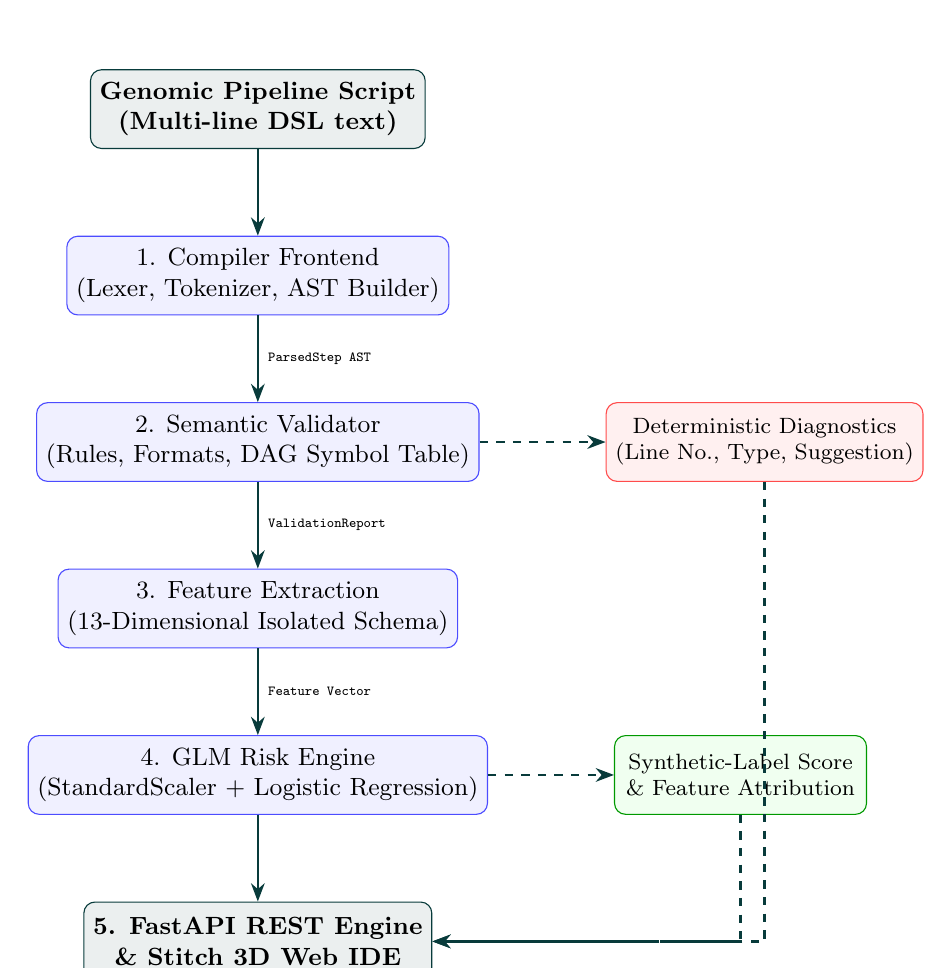
\begin{tikzpicture}[
    node distance=1.1cm and 1.5cm,
    box/.style={rectangle, draw=tealbrand, fill=tealbrand!8, rounded corners, minimum width=3.8cm, minimum height=1.0cm, align=center, font=\small\bfseries},
    proc/.style={rectangle, draw=blue!70, fill=blue!6, rounded corners, minimum width=3.8cm, minimum height=1.0cm, align=center, font=\small},
    arrow/.style={-{Stealth[scale=1.0]}, thick, draw=tealbrand}
]

% Nodes
\node[box] (input) {Genomic Pipeline Script\\(Multi-line DSL text)};
\node[proc, below=of input] (lexer) {1. Compiler Frontend\\(Lexer, Tokenizer, AST Builder)};
\node[proc, below=of lexer] (validator) {2. Semantic Validator\\(Rules, Formats, DAG Symbol Table)};
\node[proc, below=of validator] (features) {3. Feature Extraction\\(13-Dimensional Isolated Schema)};
\node[proc, below=of features] (glm) {4. GLM Risk Engine\\(StandardScaler + Logistic Regression)};
\node[box, below=of glm] (api) {5. FastAPI REST Engine\\\& Stitch 3D Web IDE};

% Lateral outputs
\node[rectangle, draw=red!70, fill=red!6, rounded corners, right=1.6cm of validator, minimum width=3.2cm, minimum height=1.0cm, align=center, font=\footnotesize] (diag) {Deterministic Diagnostics\\(Line No., Type, Suggestion)};

\node[rectangle, draw=green!60!black, fill=green!6, rounded corners, right=1.6cm of glm, minimum width=3.2cm, minimum height=1.0cm, align=center, font=\footnotesize] (telemetry) {Synthetic-Label Score\\\& Feature Attribution};

% Connections
\draw[arrow] (input) -- (lexer);
\draw[arrow] (lexer) -- node[right, font=\tiny\ttfamily] {ParsedStep AST} (validator);
\draw[arrow] (validator) -- node[right, font=\tiny\ttfamily] {ValidationReport} (features);
\draw[arrow] (features) -- node[right, font=\tiny\ttfamily] {Feature Vector} (glm);
\draw[arrow] (glm) -- (api);

\draw[arrow, dashed] (validator) -- (diag);
\draw[arrow, dashed] (glm) -- (telemetry);
\draw[arrow, dashed] (diag) |- (api);
\draw[arrow, dashed] (telemetry) |- (api);

\end{tikzpicture}
\caption{Overall System Architecture of the Intelligent Genomic Pipeline Compiler.}
\label{fig:architecture}
\end{figure}

\newpage

% ============================================================
% 4. COMPILER DESIGN AND IMPLEMENTATION
% ============================================================
\section{Compiler Design and Implementation}

\subsection{Lexical Analysis and Tokenization}

The lexical analyzer converts raw text streams into discrete lexical tokens. Unlike general-purpose languages, scientific DSLs feature command-line parameter conventions, filesystem paths containing punctuation, quoted paths with spaces, and numerical flags.

The lexer separates each non-empty command line into tokens and preserves quoted paths containing whitespace. The supported DSL includes flag-value options, numeric arguments, and comment handling. These rules are normalized before the compiler creates the parameter mapping used by semantic validation. The main lexical cases are:
\begin{enumerate}
    \item \textbf{Comment Handling:} Full-line comments beginning with \texttt{\#} or \texttt{//} are skipped; supported inline comments are removed before command parsing.
    \item \textbf{Quoted Paths:} File paths enclosed in single or double quotes (for example, \texttt{"sample 1.fq"}) are retained as a single argument.
    \item \textbf{Flag-Value Syntax:} Both separated options (\texttt{--threads 8}) and equal-sign options (\texttt{--threads=8}) are normalized into the same key-value representation.
    \item \textbf{Negative Numeric Values:} A negative value such as \texttt{-4} following an option is treated as that option's value when it matches the numeric-value rule. A negative token in an unexpected position is reported as an argument error.
    \item \textbf{Duplicate Parameters:} Repeated flags in one command are reported as a duplicate-parameter diagnostic rather than silently treated as independent values.
\end{enumerate}

\subsection{Grammar Specification and Syntax Analysis}

Listing \ref{lst:grammar} gives an EBNF-style description of the line-oriented DSL. It summarizes the structure of commands and parameters; the implementation's tokenizer and semantic validator define the exact accepted forms.

\begin{lstlisting}[language=C, caption={EBNF-style description of the line-oriented Genomic Pipeline DSL.}, label={lst:grammar}]
PipelineScript ::= { BlankLine | CommentLine | CommandStep } ;
BlankLine      ::= LineBreak ;
CommentLine    ::= CommentMarker { AnyCharacter } [LineBreak] ;
CommentMarker  ::= "#" | "//" ;
CommandStep    ::= ToolName [ SubCommand ] { Parameter } [LineBreak] ;
ToolName       ::= "FASTQC" | "TRIMMOMATIC" | "BWA"
                 | "SAMTOOLS" | "GATK" ;
SubCommand     ::= "MEM" | "INDEX" | "VIEW" | "SORT"
                 | "HAPLOTYPECALLER" | "MUTECT2"
                 | "MARKDUPLICATES" ;
Parameter      ::= LongFlag [Value] | ShortFlag [Value]
                 | LongFlag "=" Value ;
LongFlag       ::= "--" Identifier ;
ShortFlag      ::= "-" Character ;
Value          ::= QuotedString | NumberLiteral | PathOrString ;
Identifier     ::= Letter { Letter | Digit | "_" | "-" } ;
NumberLiteral  ::= [Sign] Digit { Digit } ["." Digit { Digit }] ;
Sign           ::= "+" | "-" ;
QuotedString   ::= DoubleQuoted | SingleQuoted ;
DoubleQuoted   ::= '"' { EscapedCharacter | NonQuoteCharacter } '"' ;
SingleQuoted   ::= "'" { EscapedCharacter | NonQuoteCharacter } "'" ;
PathOrString   ::= non-empty token accepted by the lexer ;
LineBreak      ::= newline ;
\end{lstlisting}

During syntax analysis, the parser constructs a sequence-level intermediate representation consisting of \texttt{ParsedStep} records. Although the report uses AST terminology for convenience, the displayed data structure is a list of command records rather than a nested tree. When parsing fails, the compiler records the corresponding diagnostic. For commands that are retained in the representation, the validity field can indicate whether the step passed frontend checks; downstream validation should avoid treating malformed steps as reliable inputs.

\subsection{Intermediate Representation (IR)}

The intermediate representation preserves semantic metadata extracted during parsing. Listing \ref{lst:parsedstep} illustrates the Pydantic schema governing \texttt{ParsedStep}.

\begin{lstlisting}[language=Python, caption={Intermediate Representation Schema (ParsedStep).}, label={lst:parsedstep}]
class ParsedStep(BaseModel):
    line_number: int
    raw_command: str
    tool: str                          # Normalized uppercase tool identifier
    subcommand: Optional[str] = None   # Subcommand identifier
    parameters: Dict[str, Any]         # Flag-value parameter mapping
    input_files: List[str]             # Inferred input file artifacts
    output_files: List[str]            # Inferred output file artifacts
    stage: str                         # Pipeline stage classification
    is_valid: bool = True              # Frontend parsing validity status
\end{lstlisting}

\subsection{Semantic Analysis and Domain Rules}

Semantic analysis ensures that structurally valid commands adhere to tool-specific computational requirements:
\begin{enumerate}
    \item \textbf{Mandatory Parameters:} Each tool possesses a required parameter specification. For example, \texttt{BWA MEM} requires \texttt{--ref}, \texttt{--in}, and \texttt{--out}. Omission triggers \texttt{MISSING\_PARAMETER}.
    \item \textbf{Parameter Formatting and File Extensions:} File parameters are verified against acceptable biological extensions. FASTQ inputs require \texttt{.fastq}, \texttt{.fq}, or compressed \texttt{.gz} variants. Reference genomes require \texttt{.fa} or \texttt{.fasta}. Alignments require \texttt{.sam} or \texttt{.bam}. Variant calls require \texttt{.vcf} or \texttt{.vcf.gz}. Numerical arguments such as \texttt{--threads} and \texttt{--minlen} must evaluate to positive integers. Trimmomatic's \texttt{--slidingwindow} requires the exact format \texttt{<window>:<quality>} (e.g., \texttt{4:20}).
    \item \textbf{Accurate Output Artifact Classification:} In \texttt{GATK MarkDuplicates}, the parameter \texttt{--metrics} generates a duplication metrics summary report. Classifying \texttt{--metrics} as an input file causes catastrophic false \texttt{UNRESOLVED\_FILE\_REFERENCE} errors; the compiler frontend registers \texttt{--metrics} as an output artifact.
\end{enumerate}

\subsection{Directed Acyclic Graph (DAG) and Symbol Table File Resolution}

To detect broken dataflows, the compiler maintains a scoped symbol table tracking produced and consumed files:
\begin{equation}
    \mathcal{S} : \text{Filename} \rightarrow \text{ProducerLineNumber}
\end{equation}
Initial pipeline inputs may be declared explicitly or inferred dynamically (e.g., raw FASTQ reads and reference FASTA files referenced in initial steps are registered at line $0$).

When an intermediate tool consumes a file, the compiler verifies $f \in \text{Domain}(\mathcal{S})$. If an unproduced file is consumed, an \texttt{UNRESOLVED\_FILE\_REFERENCE} error is emitted. Furthermore, the compiler evaluates in-place file collisions:
\begin{equation}
    \mathcal{C}_{\text{step}} = \text{input\_files} \cap \text{output\_files}
\end{equation}
If $\mathcal{C}_{\text{step}} \neq \emptyset$, an \texttt{OUTPUT\_REFERENCE\_CONFLICT} error is raised to prevent in-place file corruption. Additionally, GATK variant callers require BAM alignments to be indexed. The compiler tracks indexed BAMs; if \texttt{GATK HaplotypeCaller} accesses an unindexed BAM, an \texttt{UNINDEXED\_BAM\_INPUT} error is generated.

\subsection{Biological Workflow Sequence Matrix}

Valid pipelines do not follow a simple linear chain; they exhibit legitimate branches and parallel processing paths. For example, quality assessment (\texttt{FASTQC}) may occur before or after trimming, and reference indexing (\texttt{BWA INDEX}) may precede alignment. However, specific transitions are strictly invalid. The compiler enforces the transition rules specified in Algorithm \ref{alg:sequence_validator}.

\begin{algorithm}[H]
\caption{High-Level Workflow Validation}
\label{alg:sequence_validator}
\begin{algorithmic}[1]
\Require Parsed command records $\mathcal{P}$
\Ensure Error list $\mathcal{E}$ and warning list $\mathcal{W}$
\State Initialize $\mathcal{E},\mathcal{W} \leftarrow \emptyset$
\State Initialize flags for previously seen QC, alignment, sorting, and variant steps
\For{each step $s$ in $\mathcal{P}$, in source order}
    \State Derive the normalized tool/subcommand key and stage for $s$
    \If{$s$ is a QC step after downstream processing has begun}
        \State Add an invalid-sequence diagnostic to $\mathcal{E}$
    \EndIf
    \If{$s$ is \texttt{SAMTOOLS INDEX} and no prior sort step exists}
        \State Add an invalid-sequence diagnostic to $\mathcal{E}$
    \EndIf
    \If{$s$ is a variant-calling step and no prior alignment exists}
        \State Add an invalid-sequence diagnostic to $\mathcal{E}$
    \EndIf
    \State Update the stage and step-presence flags
\EndFor
\If{alignment or variant calling is present but QC is absent}
    \State Add a missing-QC warning to $\mathcal{W}$
\EndIf
\State \Return $\mathcal{E},\mathcal{W}$
\end{algorithmic}
\end{algorithm}

\newpage

% ============================================================
% 5. GENOMIC PIPELINE DSL AND SUPPORTED TOOLS
% ============================================================
\section{Genomic Pipeline DSL and Supported Tools}

The compiler models five principal tools spanning quality control, read alignment, alignment processing, and variant discovery. Table \ref{tab:tool_spec} documents the full DSL specification, parameter constraints, and target lifecycle stages.

\begin{table}[H]
\centering
\footnotesize
\setlength{\tabcolsep}{3pt}
\renewcommand{\arraystretch}{1.18}
\caption{Supported Genomic Tools, Command Syntax, and Parameter Specifications}
\label{tab:tool_spec}
\begin{tabularx}{\textwidth}{>{\raggedright\arraybackslash}p{2.35cm} >{\raggedright\arraybackslash}p{2.2cm} >{\raggedright\arraybackslash}p{2.45cm} >{\raggedright\arraybackslash}X >{\raggedright\arraybackslash}p{2.05cm}}
\toprule
\textbf{Tool} & \textbf{Subcommand} & \textbf{Required Flags} & \textbf{Permitted File Formats} & \textbf{Pipeline Stage} \\
\midrule
\texttt{FASTQC} & None & \texttt{--in} & In: \texttt{.fq}, \texttt{.fastq}, \texttt{.fastq.gz}\newline Out: \texttt{.html}, \texttt{.zip} & Quality Control (QC) \\
\addlinespace
\texttt{TRIMMOMATIC} & None & \texttt{--in}, \texttt{--out} & In/Out: \texttt{.fq}, \texttt{.fastq}, \texttt{.fastq.gz}\newline Flags: \texttt{--minlen}, \texttt{--slidingwindow} & Quality Control (QC) \\
\addlinespace
\texttt{BWA} & \texttt{MEM} & \texttt{--ref}, \texttt{--in}, \texttt{--out} & Ref: \texttt{.fa}, \texttt{.fasta}\newline In: FASTQ; Out: \texttt{.sam}, \texttt{.bam} & Read Alignment \\
\addlinespace
\texttt{BWA} & \texttt{INDEX} & \texttt{--ref} & Ref: \texttt{.fa}, \texttt{.fasta}, \texttt{.fna} & Reference Indexing \\
\addlinespace
\texttt{SAMTOOLS} & \texttt{VIEW} & \texttt{--in}, \texttt{--out} & In/Out: \texttt{.sam}, \texttt{.bam}\newline Flags: \texttt{-b}, \texttt{-h}, \texttt{-s} & Alignment Processing \\
\addlinespace
\texttt{SAMTOOLS} & \texttt{SORT} & \texttt{--in}, \texttt{--out} & In: \texttt{.sam}, \texttt{.bam}; Out: \texttt{.bam} & Alignment Processing \\
\addlinespace
\texttt{SAMTOOLS} & \texttt{INDEX} & \texttt{--in} & In: Coordinate-sorted \texttt{.bam} & Alignment Processing \\
\addlinespace
\texttt{GATK} & \makecell[l]{\texttt{Haplotype}\\\texttt{Caller}} & \texttt{--ref}, \texttt{--in}, \texttt{--out} & Ref: FASTA; In: Indexed \texttt{.bam}\newline Out: \texttt{.vcf}, \texttt{.vcf.gz} & Variant Calling \\
\addlinespace
\texttt{GATK} & \texttt{Mutect2} & \texttt{--ref}, \texttt{--in}, \texttt{--out} & Ref: FASTA; In: Indexed \texttt{.bam}\newline Out: \texttt{.vcf}, \texttt{.vcf.gz} & Somatic Variant Calling \\
\addlinespace
\texttt{GATK} & \makecell[l]{\texttt{Mark}\\\texttt{Duplicates}} & \texttt{--in}, \texttt{--out} & In: \texttt{.bam}; Out: \texttt{.bam}\newline Artifact: \texttt{--metrics} (\texttt{.txt}) & Alignment Processing \\
\bottomrule
\end{tabularx}
\end{table}

\subsection{Illustrative Pipeline Examples}

To clarify the concrete syntax of the genomic DSL, Listing \ref{lst:valid_pipeline} demonstrates a syntactically and semantically valid germline variant discovery pipeline.

\begin{lstlisting}[language=C, caption={A fully valid Whole Genome Sequencing (WGS) pipeline in the Genomic DSL.}, label={lst:valid_pipeline}]
// Whole-Genome Germline Variant Discovery Pipeline
FASTQC --in reads.fq --out qc_report.html --threads 4
TRIMMOMATIC --in reads.fq --out trimmed.fq --minlen 36 --slidingwindow 4:20
BWA MEM --ref hg38.fa --in trimmed.fq --out aligned.sam --threads 8
SAMTOOLS SORT --in aligned.sam --out sorted.bam --threads 4
SAMTOOLS INDEX --in sorted.bam
GATK MarkDuplicates --in sorted.bam --out dedup.bam --metrics dedup_metrics.txt
SAMTOOLS INDEX --in dedup.bam
GATK HaplotypeCaller --ref hg38.fa --in dedup.bam --out variants.vcf --threads 8
\end{lstlisting}

Conversely, Listing \ref{lst:invalid_pipeline} demonstrates a multi-fault pipeline containing syntactic, semantic, and sequence defects.

\begin{lstlisting}[language=C, caption={An invalid genomic pipeline containing multiple structural and semantic defects.}, label={lst:invalid_pipeline}]
// Inverted Trimming: Trimmomatic executed after BWA MEM (INVALID_COMMAND_SEQUENCE)
BWA MEM --ref hg38.fa --in reads.fq --out out.sam
TRIMMOMATIC --in reads.fq --out clean.fq --minlen -5  // INVALID_PARAMETER_VALUE (<0)

// Missing required parameters: SAMTOOLS SORT requires --out (MISSING_PARAMETER)
SAMTOOLS SORT --in out.sam

// Unindexed BAM consumed by GATK (UNINDEXED_BAM_INPUT)
GATK HaplotypeCaller --ref hg38.fa --in sorted.bam --out vars.vcf

// Circular overwrite hazard: reading and writing to same file (OUTPUT_REFERENCE_CONFLICT)
SAMTOOLS VIEW --in sorted.bam --out sorted.bam
\end{lstlisting}

\newpage

% ============================================================
% 6. GLM-BASED SUPPLEMENTARY RISK SCORING AND EVALUATION
% ============================================================
\section{GLM-Based Supplementary Risk Scoring and Evaluation}

\subsection{Mathematical Formulation of the GLM Classifier}

The Generalized Linear Model implements binary Logistic Regression parameterized by a weight vector $\mathbf{w} \in \mathbb{R}^{d}$ and intercept bias $b \in \mathbb{R}$. Given a standardized feature vector $\mathbf{x} \in \mathbb{R}^{d}$ extracted from a pipeline, logistic regression maps the linear predictor $\eta$ to a model output $p$. Since the training label is synthetic, $p$ is not assumed to be calibrated to real runtime failures:
\begin{align}
    \eta &= \mathbf{w}^T \mathbf{x} + b \\
    p(\text{failure} \mid \mathbf{x}) &= \sigma(\eta) = \frac{1}{1 + e^{-\eta}}
\end{align}
Model training minimizes the $L_2$-regularized negative log-likelihood objective function using the L-BFGS quasi-Newton optimization algorithm:
\begin{equation}
    \min_{\mathbf{w}, b} \frac{1}{2} \|\mathbf{w}\|_2^2 + C \sum_{i=1}^{N} \left[ -y_i \ln \sigma(\mathbf{w}^T \mathbf{x}_i + b) - (1 - y_i) \ln(1 - \sigma(\mathbf{w}^T \mathbf{x}_i + b)) \right]
\end{equation}
where $C = 1.0$ controls regularization strength. Prior to linear estimation, feature columns are centered and scaled to unit variance using \texttt{StandardScaler}:
\begin{equation}
    x_{ij}' = \frac{x_{ij} - \mu_j}{\sigma_j}
\end{equation}

\subsection{13-Dimensional Canonical Feature Schema}

The feature extraction layer maps the compiler's validation report and parsed command records to a 13-dimensional schema. Table \ref{tab:feature_schema} lists the feature definitions described by this implementation. The diagnostic-count features are not independent of the synthetic label and therefore require careful interpretation during evaluation.

\begin{table}[H]
\centering
\small
\caption{The 13 Canonical Features Extracted for the GLM Classifier}
\label{tab:feature_schema}
\begin{tabularx}{\textwidth}{p{5.0cm}p{1.8cm}X}
\toprule
\textbf{Feature Column} & \textbf{Data Type} & \textbf{Extraction Definition and Semantic Isolation} \\
\midrule
\texttt{syntax\_error\_count} & Integer $\ge 0$ & Tokenization, malformed flags, unknown commands/subcommands. \\
\makecell[l]{\texttt{missing\_parameter\_}\\\texttt{count}} & Integer $\ge 0$ & Mandatory tool parameters omitted from command step. \\
\makecell[l]{\texttt{sequence\_violation\_}\\\texttt{count}} & Integer $\ge 0$ & Out-of-order biological stage transitions. \\
\makecell[l]{\texttt{unresolved\_reference\_}\\\texttt{count}} & Integer $\ge 0$ & Intermediate files referenced before declaration or generation. \\
\makecell[l]{\texttt{file\_extension\_}\\\texttt{error\_count}} & Integer $\ge 0$ & File format mismatches (e.g., FASTQ provided where BAM required). \\
\texttt{total\_error\_count} & Integer $\ge 0$ & Aggregate sum of all errors with severity \texttt{ERROR}. \\
\texttt{warning\_count} & Integer $\ge 0$ & Non-fatal compiler warnings (e.g., missing QC stage). \\
\texttt{pipeline\_length} & Integer $\ge 1$ & Total number of parsed command steps. \\
\texttt{has\_qc\_step} & \makecell[c]{Binary\\$\{0,1\}$} & Indicator: 1 if \texttt{FASTQC} or \texttt{TRIMMOMATIC} is present. \\
\texttt{has\_alignment\_step} & \makecell[c]{Binary\\$\{0,1\}$} & Indicator: 1 if \texttt{BWA} is present. \\
\makecell[l]{\texttt{has\_variant\_calling\_}\\\texttt{step}} & \makecell[c]{Binary\\$\{0,1\}$} & Indicator: 1 if \texttt{GATK} is present. \\
\texttt{tool\_diversity\_ratio} & Float $[0, 1]$ & Ratio of unique tools to total pipeline length: $|Tools| / N_{steps}$. \\
\texttt{unindexed\_bam\_count} & Integer $\ge 0$ & Number of unindexed BAM files consumed by GATK. \\
\bottomrule
\end{tabularx}
\end{table}

\subsection{Evaluation Methodology Audit and Leakage Investigation}

During the engineering audit of the original system, the model reported $100.00\%$ accuracy, precision, recall, and ROC-AUC. An investigation was conducted into whether this performance represented true learning or experimental artifact:
\begin{enumerate}
    \item \textbf{Tautological Target Leakage:} In synthetic dataset generators, ground-truth labels are created via deterministic rule:
    \begin{equation}
        \text{failed} = \begin{cases}
            1 & \text{if } \text{total\_error\_count} > 0 \\
            0 & \text{otherwise}
        \end{cases}
    \end{equation}
    Because \texttt{total\_error\_count} was included directly in the feature matrix $\mathbf{X}$, any linear classifier learns a large positive weight on this single column ($\beta_{\text{total\_errors}} = +4.1956$), rendering the classification trivial.
    \item \textbf{Data Leakage via Mutation Clones:} Generating mutants by injecting single errors into identical pipeline templates results in train and test sets sharing identical syntactic backbones. Random shuffling (\texttt{train\_test\_split}) leaks structural templates across splits.
\end{enumerate}

To reduce these risks and make the evaluation easier to interpret:
\begin{itemize}
    \item \textbf{Group-Isolated Partitioning:} The dataset of 240 samples was partitioned into 12 distinct structural template groups (\texttt{GRP\_01} to \texttt{GRP\_12}). Using \texttt{GroupShuffleSplit}, 9 entire template families (180 samples) were assigned to training, and 3 complete families (60 samples) were held out for testing, with \textbf{$0.00\%$ template-group overlap}. This controls template reuse but does not, on its own, eliminate target leakage from diagnostic features.
    \item \textbf{Ablated Benchmark Control:} An ablated model was evaluated after removing \texttt{total\_error\_count}. This removes the direct aggregate feature, but individual diagnostic counts can still be strongly associated with the label because the label itself is derived from compiler errors. The ablation should therefore not be described as eliminating all target dependence.
\end{itemize}

For traceability, the SHA-256 digest of \path{backend/data/train_dataset.json} in the reviewed archive is \texttt{\seqsplit{9671d9fe74e86e15f7175e76235225ea771caa5bdd18bf0688865b7fc9580827}}. The persisted model metadata records the same dataset digest. This ties the stored evaluation summary to this dataset file, but does not establish that the synthetic labels represent real execution outcomes.

\subsection{Experimental Results and Baseline Comparison}

Table \ref{tab:eval_results} summarizes the results recorded for four classifiers on the reported 60-sample synthetic holdout, along with a three-fold group-stratified cross-validation summary. The figures should be read as results for the synthetic static-validity label, not for runtime failures on real genomic workloads.

\begin{table}[H]
\centering
\footnotesize
\setlength{\tabcolsep}{3pt}
\renewcommand{\arraystretch}{1.18}
\caption{Reported classification results for the synthetic static-validity label (60-sample holdout)}
\label{tab:eval_results}
\begin{tabularx}{\textwidth}{>{\raggedright\arraybackslash}X *{5}{>{\centering\arraybackslash}p{1.4cm}}}
\toprule
\textbf{Model / Evaluation Protocol} & \makecell{\textbf{Accu-}\\\textbf{racy}} & \makecell{\textbf{Preci-}\\\textbf{sion}} & \textbf{Recall} & \makecell{\textbf{F1-}\\\textbf{Score}} & \makecell{\textbf{Brier}\\\textbf{Score}} \\
\midrule
Majority-class baseline (Dummy) & 0.5000 & 0.0000 & 0.0000 & 0.0000 & 0.5000 \\
Deterministic rule (\texttt{errors > 0}) & 1.0000 & 1.0000 & 1.0000 & 1.0000 & N/A \\
Full GLM (all 13 features) & 1.0000 & 1.0000 & 1.0000 & 1.0000 & 0.0154 \\
Ablated GLM (excluding aggregate error count) & \textbf{0.9333} & \textbf{1.0000} & \textbf{0.8667} & \textbf{0.9286} & \textbf{0.0808} \\
\bottomrule
\end{tabularx}
\end{table}

\noindent\footnotesize\textit{Cross-validation summary:} The recorded 3-fold group-stratified run on 180 training samples reported mean accuracy of $96.67\%$ with a standard deviation of 2.72 percentage points.\\[2pt]\textit{Interpretation:} The target label is defined from static compiler errors. The deterministic rule's perfect score is therefore expected by construction, and the full GLM includes the aggregate error-count feature used to define that label. The Brier scores are descriptive values on this synthetic holdout; they do not establish calibration for real runtime failures.\normalsize

\subsection{Small Independent Template Benchmark}

A separate set of 15 manually designed pipeline examples (\path{independent_eval_set.json}) was used as a small additional check. Although these examples were created separately from the training templates, they are still synthetic examples and are too few to support broad claims about out-of-distribution generalization:
\begin{itemize}
    \item \textbf{Deterministic Compiler Rule:} Classified all 15 examples correctly (7 valid and 8 invalid).
    \item \textbf{Full GLM Model:} $100.00\%$ accuracy, F1-score $= 1.0000$.
    \item \textbf{Ablated GLM Model:} Achieved \textbf{$80.00\%$ accuracy} and \textbf{$0.8421$ F1-score} (12/15 correct classifications, precision $= 0.7273$, recall $= 1.0000$).
\end{itemize}

\subsection{Learned Feature Coefficients and Log-Odds Impact}

Inspection of the GLM weight vector provides statistical transparency. Figure \ref{fig:coefficients} visualizes the standardized logistic regression coefficients.

\begin{figure}[H]
\centering
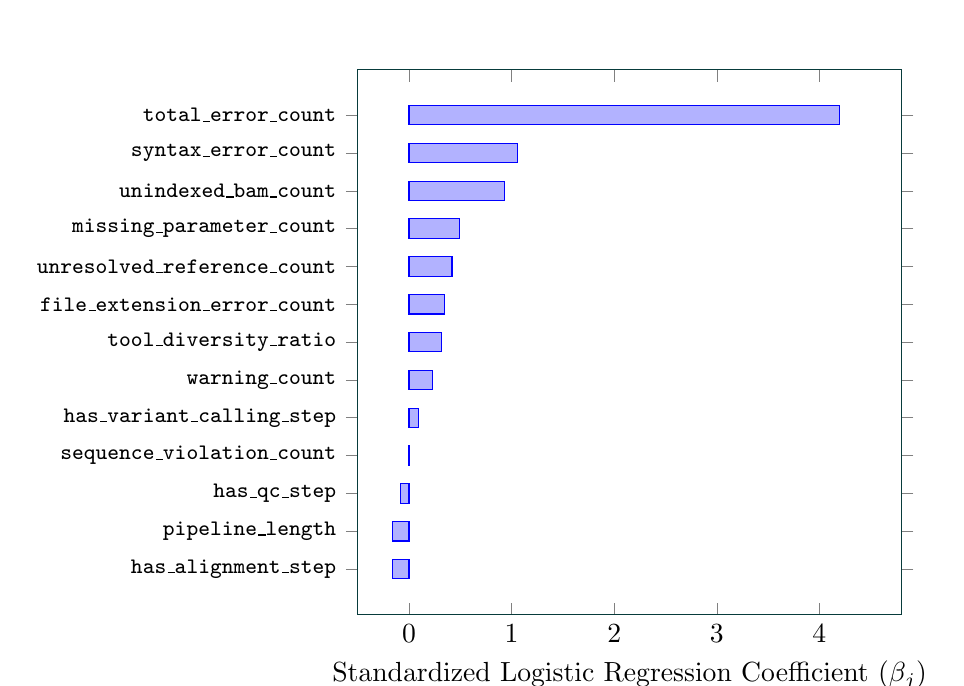
\begin{tikzpicture}
\begin{axis}[
    xbar,
    width=0.70\textwidth,
    height=8.5cm,
    xlabel={Standardized Logistic Regression Coefficient ($\beta_j$)},
    symbolic y coords={
        has_align,
        pipe_len,
        has_qc,
        seq_viol,
        has_var,
        warn_cnt,
        tool_div,
        file_ext,
        unres_ref,
        miss_param,
        unidx_bam,
        synt_err,
        tot_err
    },
    ytick=data,
    yticklabels={
        \texttt{total\_error\_count},
        \texttt{syntax\_error\_count},
        \texttt{unindexed\_bam\_count},
        \texttt{missing\_parameter\_count},
        \texttt{unresolved\_reference\_count},
        \texttt{file\_extension\_error\_count},
        \texttt{tool\_diversity\_ratio},
        \texttt{warning\_count},
        \texttt{has\_variant\_calling\_step},
        \texttt{sequence\_violation\_count},
        \texttt{has\_qc\_step},
        \texttt{pipeline\_length},
        \texttt{has\_alignment\_step}
    },
    yticklabel style={font=\footnotesize},
    xmin=-0.5, xmax=4.8,
    bar width=7pt,
    fill=tealbrand!75,
    draw=tealbrand
]
\addplot coordinates {
    (4.1956,tot_err)
    (1.0599,synt_err)
    (0.9282,unidx_bam)
    (0.4912,miss_param)
    (0.4194,unres_ref)
    (0.3419,file_ext)
    (0.3183,tool_div)
    (0.2321,warn_cnt)
    (0.0895,has_var)
    (-0.0085,seq_viol)
    (-0.0788,has_qc)
    (-0.1621,pipe_len)
    (-0.1640,has_align)
};
\end{axis}
\end{tikzpicture}
\caption{Learned Logistic Regression Coefficients ($\beta_j$) for the 13 Feature Dimensions.}
\label{fig:coefficients}
\end{figure}

In the recorded model, positive coefficients increase the model's score for the synthetic positive class and negative coefficients decrease it, holding other features fixed. Because the target is derived from static error counts, these coefficients describe associations within the synthetic dataset; they should not be interpreted as evidence that the features cause or predict real execution failures.

\newpage

% ============================================================
% 7. BACKEND API AND FRONTEND INTEGRATION
% ============================================================
\section{Backend API and Frontend Integration}

\subsection{FastAPI REST Architecture}

The backend service is engineered with FastAPI and served via Uvicorn. The API exposes five REST endpoints:
\begin{enumerate}
    \item \texttt{GET /health}: Evaluates service health, memory readiness, loaded scikit-learn model version, and supported toolsets.
    \item \texttt{POST /analyze}: Accepts raw pipeline text and optional declared inputs. Returns parsed AST steps, deterministic validation reports, extracted 13D features, and GLM risk predictions.
    \item \texttt{POST /predict}: Accepts either raw script text or an arbitrary feature dictionary, performing input sanitization against \texttt{NaN}, \texttt{inf}, and out-of-range bounds.
    \item \texttt{GET /samples}: Returns 7 pre-compiled benchmark pipelines illustrating valid workflows and diverse error categories.
    \item \texttt{GET /docs}: Interactive Swagger OpenAPI documentation.
\end{enumerate}

The reported implementation includes a CORS configuration, a request-size guard, and centralized exception handling. These measures are useful safeguards, but a security claim should be based on the actual configuration and tests for the release being submitted; the prototype has not undergone a formal security audit.

\subsection{Web Developer Interface}

The frontend is implemented as a single-page web interface with a light page layout and a dark code-editor workspace. Key architectural components include:
\begin{itemize}
    \item \textbf{Three.js 3D DNA Double Helix:} A real-time WebGL canvas rendering a rotating DNA double helix reacting to mouse movement and viewport changes.
    \item \textbf{Code Editor Workspace:} Line-number gutter, character counters, tab indentation support, and compilation keyboard shortcuts (\texttt{Ctrl+B} / \texttt{Cmd+B}).
    \item \textbf{Execution DAG Visualizer:} Graphically renders the linearized dependency pipeline showing tool subcommands, consumed files, and output artifacts.
    \item \textbf{Telemetry Risk Meter:} An interactive SVG gauge displaying experimental synthetic-label score (0.00 to 1.00), operational risk tiers (LOW, MEDIUM, HIGH), and top contributing factors.
\end{itemize}

\newpage

% ============================================================
% 8. TESTING AND EXPERIMENTAL VERIFICATION
% ============================================================
\section{Testing and Experimental Verification}

\subsection{Automated Test Suite Breakdown}

The supplied project archive was tested by running the following command from the project root:
\begin{lstlisting}[numbers=none,frame=single,basicstyle=\ttfamily\small]
PYTHONPATH=backend pytest backend/tests -q
\end{lstlisting}
The run completed with \textbf{62 passed in 1.71 seconds} across six test modules. The review environment used scikit-learn 1.8.0, while the project requirements and saved model artifact specify scikit-learn 1.9.1; the run therefore emitted 60 estimator-version warnings while loading the persisted model. The passing test result is reproducible in this review environment, but a final submission check should also be run in an environment that matches the pinned dependency versions.

\begin{table}[H]
\centering
\footnotesize
\setlength{\tabcolsep}{4pt}
\renewcommand{\arraystretch}{1.15}
\caption{pytest Test Suite Execution Summary for the Reviewed Archive}
\label{tab:test_suite}
\begin{tabularx}{\textwidth}{>{\raggedright\arraybackslash}p{3.8cm}c>{\raggedright\arraybackslash}X}
\toprule
\textbf{Test Module} & \textbf{Pass Count} & \textbf{Verification Scope and Edge Cases Covered} \\
\midrule
\texttt{test\_compiler.py} & 20 & Valid pipelines, missing/unknown subcommands, quoted spaces, \texttt{--flag=value}, negative parameters, duplicate flags, comments, workflow transitions, circular conflicts. \\
\addlinespace
\texttt{test\_api.py} & 14 & Health, valid/invalid and empty analysis requests, request-size limits, prediction payload validation, samples/docs endpoints, CORS, frontend serving. \\
\addlinespace
\texttt{test\_features.py} & 9 & Schema column ordering, single-source error isolation, dictionary validation, rejection of \texttt{NaN}, \texttt{inf}, negative counts, and invalid ratios. \\
\addlinespace
\texttt{test\_model.py} & 7 & Artifact loading and metadata, missing/corrupted artifact handling, positive-class resolution, valid/faulty pipeline scoring, feature-dictionary prediction. \\
\addlinespace
\texttt{test\_evaluation.py} & 7 & Group isolation ($0\%$ overlap), leakage detection, independent benchmark evaluation, schema parity, baseline metadata persistence. \\
\addlinespace
\texttt{test\_dataset.py} & 5 & Dataset size/balance, static error verification ($0$ errors for valid, $>0$ for invalid), absence of contradictory labels, metadata completeness. \\
\midrule
\textbf{Total} & \textbf{62/62} & Review run: 62 passed in 1.71 s; 60 scikit-learn version warnings (see text). \\
\bottomrule
\end{tabularx}
\end{table}

\subsection{Latency and Computational Overhead}

No reproducible latency benchmark script or raw timing log was found in the archive; therefore, this report makes no quantitative latency claim.

\newpage

% ============================================================
% 9. DISCUSSION AND LIMITATIONS
% ============================================================
\section{Discussion and Limitations}

\subsection{Architectural Synthesis: Determinism vs. Probability}

A vital pedagogical and practical insight of this project is the strict boundary between deterministic compilation and statistical inference. The compiler applies deterministic rules to the parts of the pipeline language it supports: if a command references an unindexed BAM, that constraint is violated with mathematical certainty. The GLM machine learning classifier cannot replace this deterministic verification; rather, its utility lies in:
\begin{itemize}
    \item \textbf{Continuous Risk Scoring:} Generating a smooth operational risk metric for complex workflows containing non-fatal warnings and high structural complexity.
    \item \textbf{Cross-Pipeline Telemetry:} Allowing bioinformatics administrators to aggregate and prioritize hundreds of user scripts in shared HPC queues based on risk scores.
\end{itemize}

\subsection{Known Limitations and Scope Boundaries}

To maintain rigorous scientific integrity, several explicit limitations must be noted:
\begin{enumerate}
    \item \textbf{Synthetic Evaluation Distribution:} Model training and evaluation rely on verified synthetic mutations. The group split reduces repeated-template overlap, but individual diagnostics remain related to the target by construction. Performance on real workflows has not been established.
    \item \textbf{No Runtime Execution Simulation:} The compiler performs static analysis of syntax, parameters, and DAG dependencies. It does not execute the underlying Multi-gigabyte binaries or simulate cluster runtime hardware faults (e.g., node out-of-memory errors, disk quota exhaustion, or corrupted FASTA binary structures).
    \item \textbf{Simplified Tool Interfaces:} The DSL models the primary parameters of the supported tools; highly specialized flags of proprietary tool distributions are not modeled.
\end{enumerate}

\newpage

% ============================================================
% 10. CONCLUSION AND FUTURE WORK
% ============================================================
\section{Conclusion and Future Work}

\subsection{Conclusion}

This project presents a compiler-oriented prototype for checking genomic pipeline scripts before execution. Its main contribution is the separation of deterministic static validation from a supplementary GLM score. The compiler applies the syntax and semantic rules defined for the supported DSL, including selected parameter checks, file-dependency checks, BAM-index verification, and workflow-order diagnostics. These checks can identify known configuration problems before a pipeline is submitted, but they cannot guarantee successful execution on real compute infrastructure.

The recorded evaluation compares a deterministic error-count rule with full and ablated logistic-regression models on synthetic static-validity labels. Re-running the supplied training script reproduced $96.67\%$ mean accuracy (standard deviation $2.72$ percentage points) for three-fold group-stratified cross-validation on the 180-sample training split, $93.33\%$ accuracy for the ablated model on the 60-sample grouped holdout, and $80.00\%$ accuracy for the ablated model on the separate 15-example set. The full model and deterministic rule both scored $100.00\%$ on static validity, as expected from the label definition. The ablation removes the aggregate count but not all dependence between compiler diagnostics and the synthetic label, so the results do not establish prediction of real-world genomic execution failures. The supplied test suite passed 62 tests in the review environment; because that environment used a different scikit-learn version from the pinned project dependency, the final environment-specific test should be repeated before submission. No reproducible latency measurement was found in the archive, so performance claims are left for future measured evaluation.

\subsection{Future Work}

Future extensions to this research include:
\begin{enumerate}
    \item \textbf{WMS Parser Frontends:} Developing grammar parsers for Nextflow and Snakemake scripts to extract DAGs directly from industry-standard workflow definitions.
    \item \textbf{Language Server Protocol (LSP) Implementation:} Packaging the compiler frontend into an LSP service to provide live diagnostic squiggles and auto-complete in VS Code.
    \item \textbf{Empirical Runtime Telemetry:} Training GLMs on historical cluster Slurm accounting logs to correlate static compiler metrics with empirical node failure rates.
\end{enumerate}

\newpage

% ============================================================
% REFERENCES
% ============================================================
\begin{thebibliography}{99}

\bibitem{aho2006}
A. V. Aho, M. S. Lam, R. Sethi, and J. D. Ullman,
\textit{Compilers: Principles, Techniques, and Tools},
2nd ed., Boston, MA: Pearson / Addison-Wesley, 2006.

\bibitem{cooper2011}
K. D. Cooper and L. Torczon,
\textit{Engineering a Compiler},
2nd ed., San Francisco, CA: Morgan Kaufmann, 2011.

\bibitem{mckenna2010}
A. McKenna, M. Hanna, E. Banks, A. Sivachenko, K. Cibulskis, A. Kernytsky, K. Garimella, D. Altshuler, S. Gabriel, M. Daly, and M. A. DePristo,
``The Genome Analysis Toolkit: A MapReduce framework for analyzing next-generation DNA sequencing data,''
\textit{Genome Research}, vol. 20, no. 9, pp. 1297--1303, 2010.

\bibitem{li2009}
H. Li, B. Handsaker, A. Wysoker, T. Fennell, J. Ruan, N. Homer, G. Marth, G. Abecasis, R. Durbin, and 1000 Genome Project Data Processing Subgroup,
``The Sequence Alignment/Map format and SAMtools,''
\textit{Bioinformatics}, vol. 25, no. 16, pp. 2078--2079, 2009.

\bibitem{li2009b}
H. Li and R. Durbin,
``Fast and accurate short read alignment with Burrows-Wheeler transform,''
\textit{Bioinformatics}, vol. 25, no. 14, pp. 1754--1760, 2009.

\bibitem{bolger2014}
A. M. Bolger, M. Lohse, and B. Usadel,
``Trimmomatic: a flexible trimmer for Illumina sequence data,''
\textit{Bioinformatics}, vol. 30, no. 15, pp. 2114--2120, 2014.

\bibitem{andrews2010}
S. Andrews,
``FastQC: A quality control tool for high throughput sequence data,''
Babraham Bioinformatics, Babraham Institute, Cambridge, UK, 2010.

\bibitem{vanderauwera2020}
G. A. Van der Auwera and B. D. O'Connor,
\textit{Genomics the Cloud: Using Docker, GATK, and WDL in Terra},
Sebastopol, CA: O'Reilly Media, 2020.

\bibitem{ditommaso2017}
P. Di Tommaso, M. Chatzou, E. W. Floden, P. P. Barja, E. Palumbo, and C. Notredame,
``Nextflow enables reproducible computational workflows,''
\textit{Nature Biotechnology}, vol. 35, no. 4, pp. 316--319, 2017.

\bibitem{koster2012}
J. K{\"o}ster and S. Rahmann,
``Snakemake---a scalable bioinformatics workflow engine,''
\textit{Bioinformatics}, vol. 28, no. 19, pp. 2520--2522, 2012.

\bibitem{amstutz2016}
P. Amstutz, M. R. Crusoe, N. Tijani{\'c}, B. Chapman, J. Chilton, M. Heuer, A. Kartashov, D. Leehr, H. M{\'e}nager, M. Nedeljkovich, and M. Scales,
``Common Workflow Language, v1.0,''
\textit{Figshare}, Specification, 2016.

\bibitem{nelder1972}
J. A. Nelder and R. W. Wedderburn,
``Generalized linear models,''
\textit{Journal of the Royal Statistical Society: Series A (General)}, vol. 135, no. 3, pp. 370--384, 1972.

\bibitem{pedregosa2011}
F. Pedregosa, G. Varoquaux, A. Gramfort, V. Michel, B. Thirion, O. Grisel, M. Blondel, P. Prettenhofer, R. Weiss, V. Dubourg, and J. Vanderplas,
``Scikit-learn: Machine learning in Python,''
\textit{Journal of Machine Learning Research}, vol. 12, pp. 2825--2830, 2011.

\bibitem{cousot1977}
P. Cousot and R. Cousot,
``Abstract interpretation: a unified lattice model for static analysis of programs by construction or approximation of fixpoints,''
in \textit{Proc. 4th ACM SIGACT-SIGPLAN Symposium on Principles of Programming Languages (POPL)}, 1977, pp. 238--252.

\bibitem{chidamber1994}
S. R. Chidamber and C. F. Kemerer,
``A metrics suite for object oriented design,''
\textit{IEEE Transactions on Software Engineering}, vol. 20, no. 6, pp. 476--493, 1994.

\end{thebibliography}

\end{document}